\thispagestyle{plain}
~\phantom{a}

\vskip .5cm

\begin{center}
{\includegraphics[scale=1.5]{om.eps}}\\[5pt]

{\large ಅಮರವಾಣೀ}\\[5pt]

{\Large (ಶ್ರೀರಂಗಮಹಾಗುರುಗಳ ಪ್ರವಚನಗಳ ಸಂಕಲನ )}\\[5pt]

{\large ಸಂಪುಟ -೧೨}\\[5pt]

{\large ವೇದಾಂಗಗಳು -ದರ್ಶನ - ಇತಿಹಾಸಪುರಾಣ}

\end{center}

\vskip 10pt

\begin{figure}[h]
\centerline
{\includegraphics[scale=.18]{0000a.eps}}
\end{figure}


\vskip -10pt

\begin{center}

{\large ಅಷ್ಟಾಂಗಯೋಗವಿಜ್ಞಾನಮಂದಿರಂ}

{\normalsize ೯೫೭, ಶ್ರೇಷಾದ್ರಿ ಅಯ್ಯರ್ ರಸ್ತೆ,}

{\normalsize ಲಕ್ಷ್ಮ್ನೀಪುರಮ್, ಮೈಸೂರು-೪}

\end{center}

\newpage

\begin{figure}[h]
\centerline
{\includegraphics[scale=.18]{0000b.eps}}
\end{figure}

\begin{center}
{\includegraphics[scale=1.5]{om.eps}}\\[5pt]

{\large ಅಮರವಾಣೀ}\\[5pt]

{\normalsize ಸಂಪುಟ-೧೨}\\[5pt]

{\large ವೇದಾಂಗಗಳು-ದರ್ಶನ -ಇತಿಹಾಸಪುರಾಣ}\\[5pt]

{\normalsize (ಶ್ರೀರಂಗಮಹಾಗುರುಗಳ ಪ್ರವಚನಗಳ ಸಂಕಲನ)}
\end{center}

\vskip 5cm

\begin{center}
{\large ಶ್ರೀರಂಗಮಹಾಗುರು}
\end{center}

\newpage

{\eng AMARAVANI -XII : Vedangagalu -Darshana -Ithihasa purana-by Sriranga Mahaguru:published by Astanga Yoga Vijnana Mandiram, 957, Seshadri Iyer Road, Laxmipuram, Mysuru 4}

\medskip
{\eng pp. ??????}%xvi+272+68}

\medskip
{\eng First Edition May 1998}

\medskip

ಗ್ರಂಥದ ಸ್ವಾಮ್ಯ ಪ್ರಕಾಶಕರಿಗೆ ಸೇರಿದ

\vskip 3cm
\begin{center}
ಮೌಲ್ಯ :

ಸಾಧಾರನ ಪ್ರತಿ ರೂ.

ಉತ್ತಮ ಪ್ರತಿ ರೂ.
\end{center}

\vskip 2cm

\begin{center}
ಅಷ್ಟಾಂಗಯೋಗವಿಜ್ಞಾನಮಂದಿರದ ಖಾಖೆಗಳು :

\medskip
೬೨೫, ೪ನೆ ಕ್ರಾಸ್ \hspace{1cm}  ಶ್ರೀಸದ್ಗುರುವಿದ್ಯಾಶಾಲಾ

\medskip
ಹನುಮಂತನಗರ \hspace{2.5cm} ಬಸರೀಕಟ್ಟೆ

\medskip
ಬೆಂಗಳೂರು ೧೯ \hspace{1.3cm} ಚಿಕ್ಕಮಗಳೂರು ಜಿಲ್ಲೆ
\end{center}

\vskip 2cm

\begin{center}
ಮುದ್ರಣ :

ಚಂಚು ಪ್ರೆಸ್, ಮೈಸೂರು

ದೂರವಾಣಿ {\rm 61558}
\end{center}
